\subsection{View}
The \emph{view}, which serves as the user interface, provides an interface for the user to interact with the application. The \emph{view} will be implemented as a graphical user interface (GUI) to enhance the user experience. 
It is responsible for displaying the pre-defined functionalities in \autoref{chap:model_design}, allowing users to easily navigate and use the features provided by the application. 
Several mock-ups have been designed using the UI design tool UIzard\footnote{UIzard is a UI design tool used for designing wireframes, mockups, and prototypes. Homepage: \url{https://uizard.io/}} to provide a clearer visualization of the layout of the user interface.

\subsubsection{HomeFragment}
The \emph{HomeFragment} serves as the main screen of the application, providing an overview of the user's health and activity-related functionalities defined in \autoref{chap:hr_monitor_design}. This \emph{view} consists of various components, including real-time heart rate display and activity monitor.
The real-time heart rate display dynamically shows the user's live heart rate, allowing them to track their cardiovascular activity. Additionally, it features a dynamic graph that visualizes the user's heart rate history, which enables them to track their heart rate patterns over time.
The activity monitor informs the user's current activity intensity based on their current heart rate, which enables them to track their activity intensity and adjust their current activity intensity according to their needs. As mentioned in \autoref{chap:activity_intensity}, the intensity levels range from very light, light, moderate, hard, and very hard.

\begin{figure}[H]
    \centering
    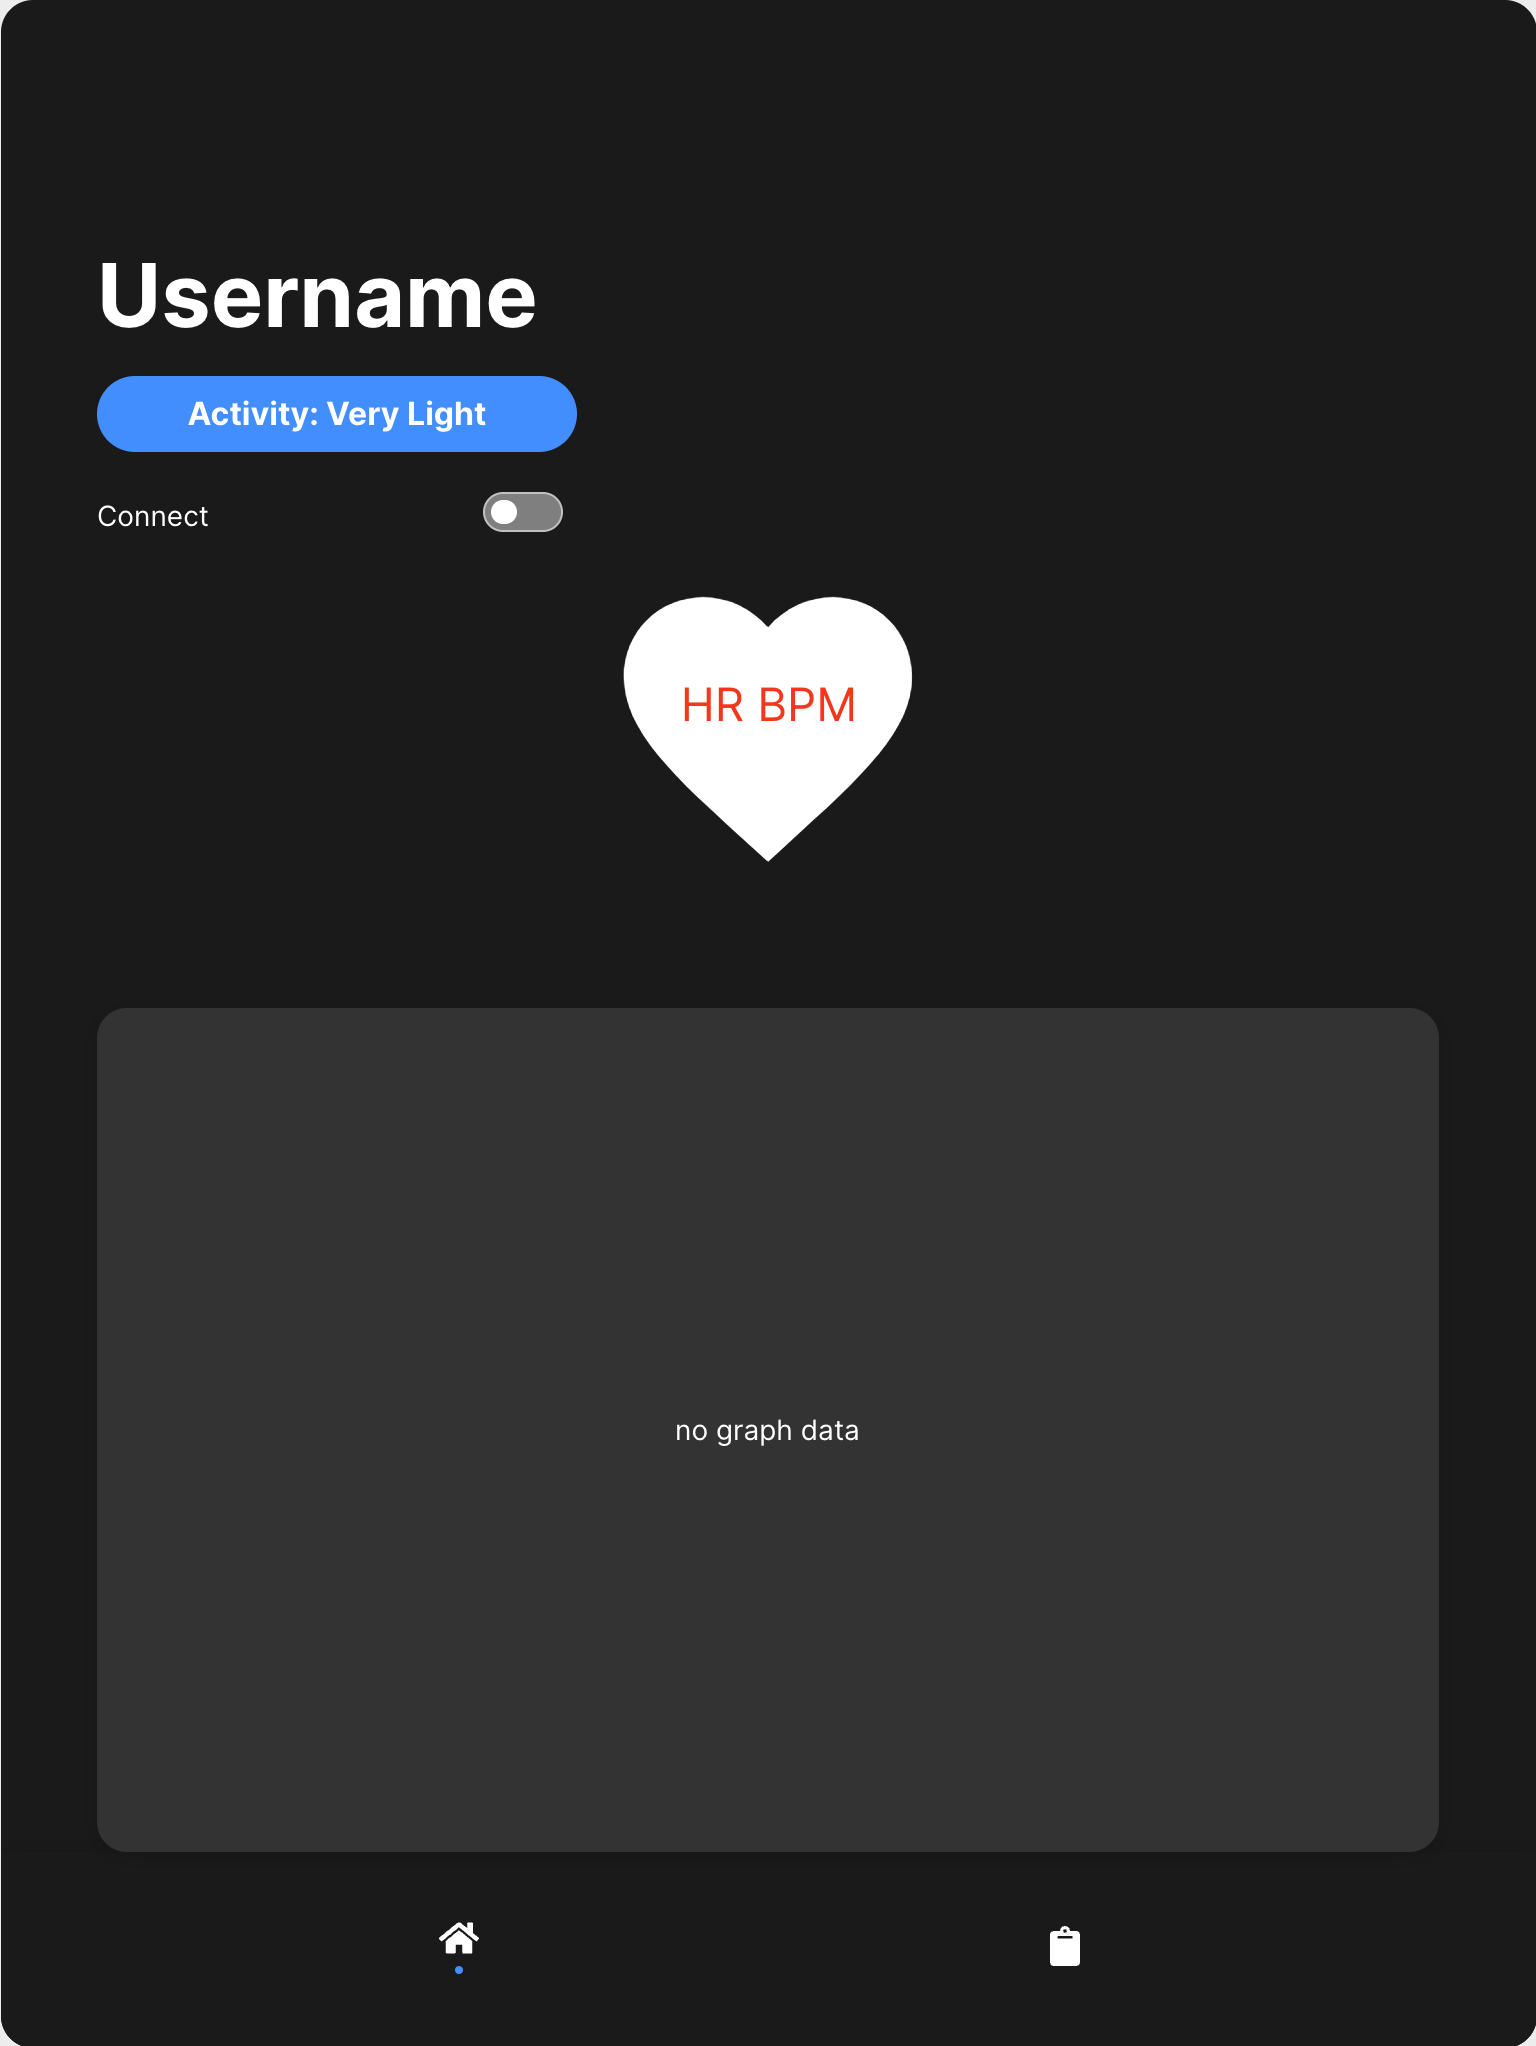
\includegraphics[width=0.75\textwidth]{images/home-fragment-mockup.png}
    \caption{HomeFragment mock-up}
    \label{fig:homefragment_mockup}
\end{figure}

As part of the real-time tracking and display of heart rate and current activity, the following sequence is executed:
\begin{enumerate}
    \item A switch is pressed to connect the application to the heart rate sensor.
    \item A request to start connection service is sent to the \emph{ConnectionServiceManager}.
    \item The \emph{ConnectionService} is started.
    \item \emph{HomeFragment} actively observes the heart rate live data from \emph{HrViewModel}.
    \item \emph{HomeFragment} actively observes the current activity live data from \emph{HrViewModel}.
    \item when the values from both the live data change, \emph{HomeFragment} is notified.
    \item \emph{HomeFragment} updates the UI according to the data changes.

\end{enumerate}

\begin{figure}[H]
    \centering
    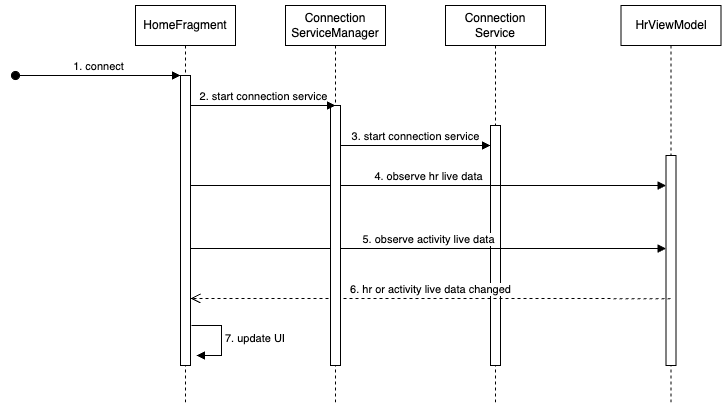
\includegraphics[width=1\textwidth]{diagrams/hr-broadcast-homefragment.drawio.png}
    \caption{HomeFragment sequence diagram}
    \label{fig:homefragment_diagram}
\end{figure}

As part of the requirements, the user interface must facilitate the functionality to stop the connection between the application and the heart rate sensor. Therefore, the following sequence is needed:
\begin{enumerate}
    \item A switch is pressed to disconnect the application to the heart rate sensor.
    \item A request to stop connection service is sent to the \emph{ConnectionServiceManager}.
    \item The \emph{ConnectionService} is stopped.
    \item \emph{HomeFragment} updates the UI accordingly.
\end{enumerate}

\begin{figure}[H]
    \centering
    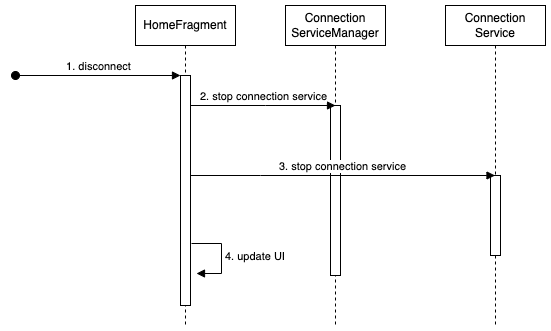
\includegraphics[width=1\textwidth]{diagrams/stop-connection-service-homefragment.drawio.png}
    \caption{HomeFragment stop connection sequence diagram}
    \label{fig:homefragment_stop_connection_diagram}
\end{figure}


\subsubsection{ExerciseFragment}
The \emph{ExerciseFragment} serves as the main component for presenting exercise details and displaying the calculation of energy expenditure. 
It shows an overview of the exercise, allowing users to access relevant information.
As part of calculating the energy expenditure, the \emph{ExerciseFragment} facilitates intuitive controls to start and stop the exercise so that the data can be captured effectively. As a result, the following sequence is executed:

\begin{enumerate}
    \item A button is pressed to start the exercise.
    \item A request to start the exercise is sent to the \emph{ExerciseServiceManager}.
    \item The \emph{ExerciseService} is started.
    \item \emph{HomeFragment} actively observes the exercise live data from \emph{ExerciseViewModel}.
    \item When the values from the live data change, \emph{ExerciseFragment} is notified.
    \item \emph{ExerciseFragment} updates the UI according to the data changes.
    \item A button is pressed to stop the exercise.
    \item A request to stop the exercise is sent to the \emph{ExerciseServiceManager}.
    \item The \emph{ExerciseService} is stopped.
    \item \emph{ExerciseFragment} updates the UI accordingly.
\end{enumerate}

\begin{figure}[H]
    \centering
    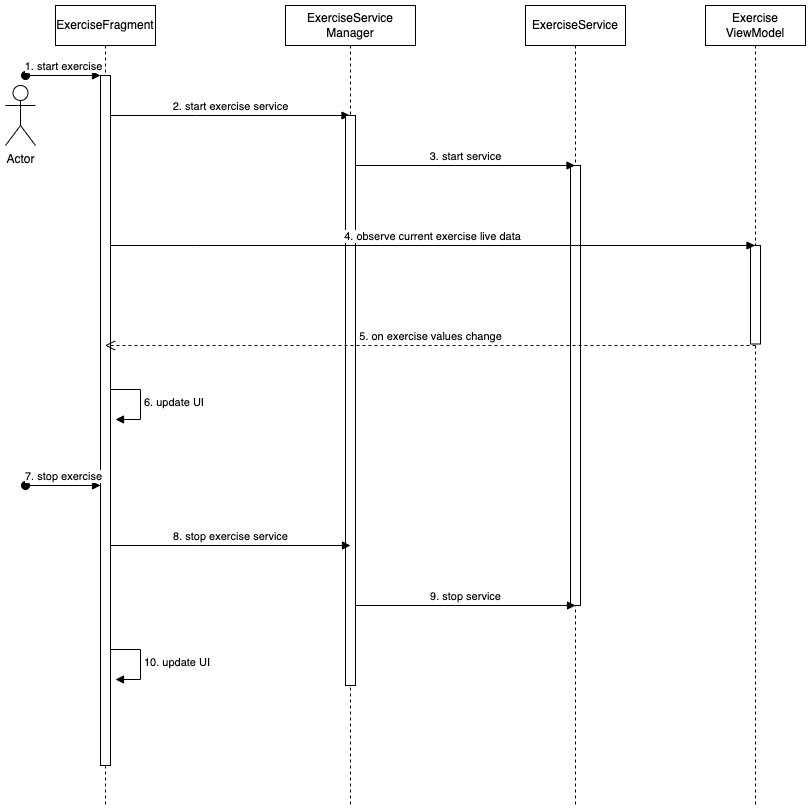
\includegraphics[width=1\textwidth]{diagrams/start-ex-frag.drawio.png}
    \caption{ExerciseFragment start exercise sequence diagram}
    \label{fig:exercisefragment_start_diagram}
\end{figure}


\begin{figure}[H]
    \centering
    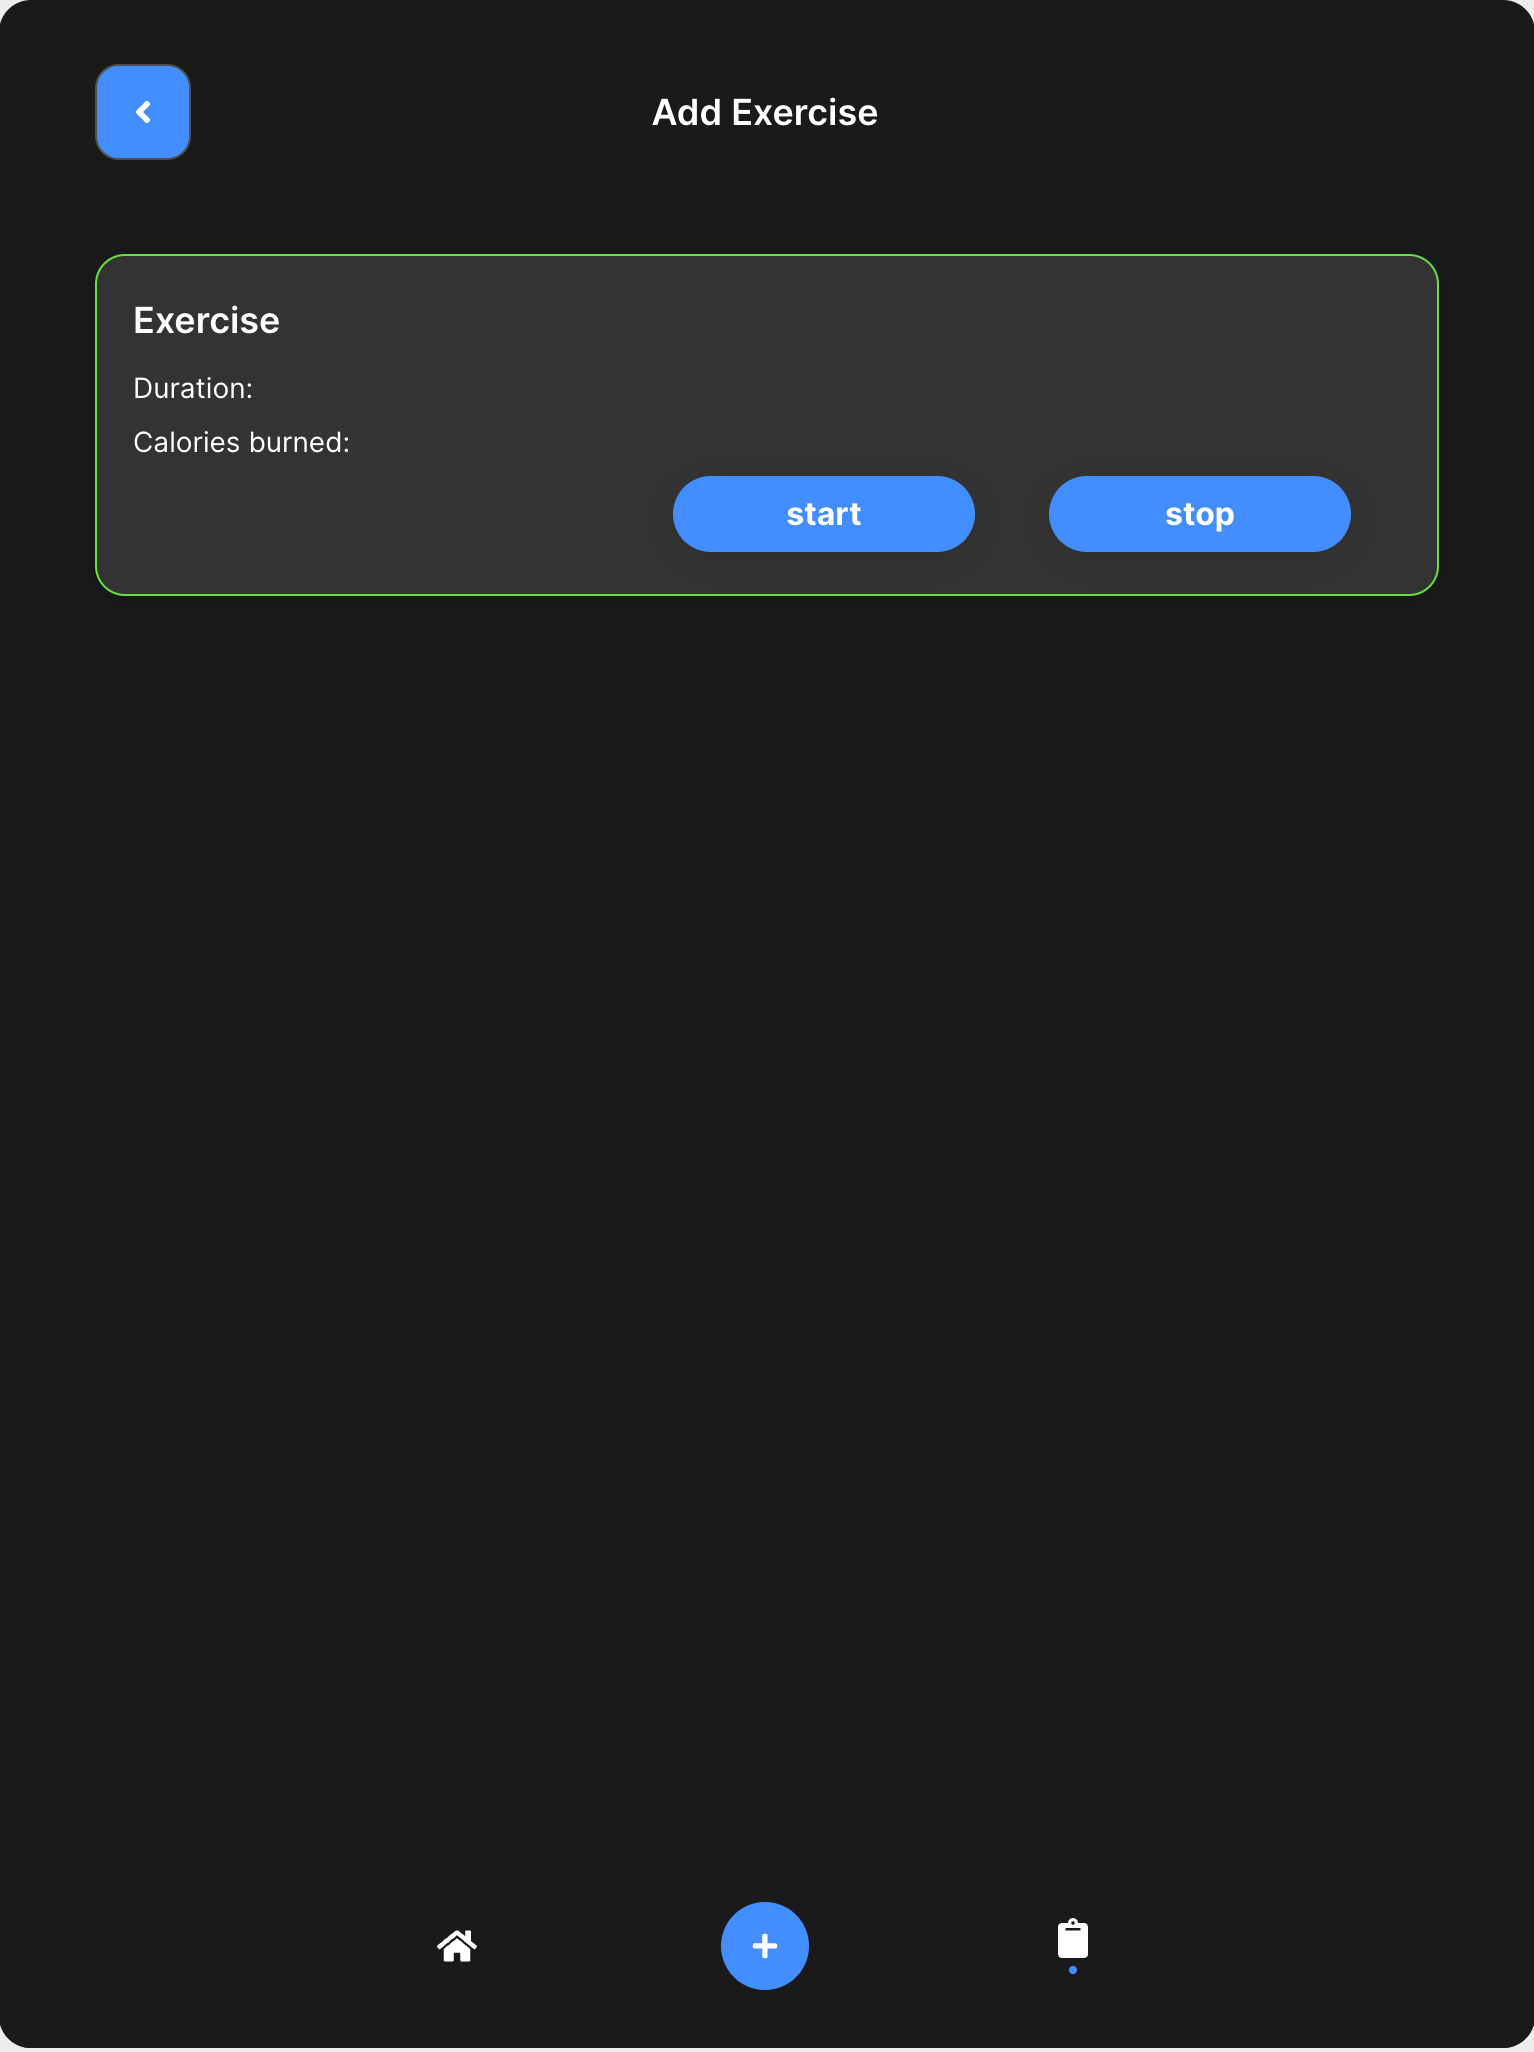
\includegraphics[width=0.75\textwidth]{images/exercise-fragment-mockup.png}
    \caption{ExerciseFragment mock-up}
    \label{fig:exercisefragment_mockup}
\end{figure}

\subsubsection{UserFragment}
The \emph{UserFragment} serves as the main component for managing user-related information. 
The \emph{UserFragment} presents an overview of the user's data, allowing users to view and manage their data conveniently. 
It offers an organized and user-friendly display, enabling users to access their profile and manage their data, including deleting their data.
The user data is displayed in a user-friendly and editable format within a TextField. This allows users to view and conveniently modify their data. 
The TextField provides a responsive and interactive interface, enabling users to easily input or update their information. 

\begin{figure}[H]
    \centering
    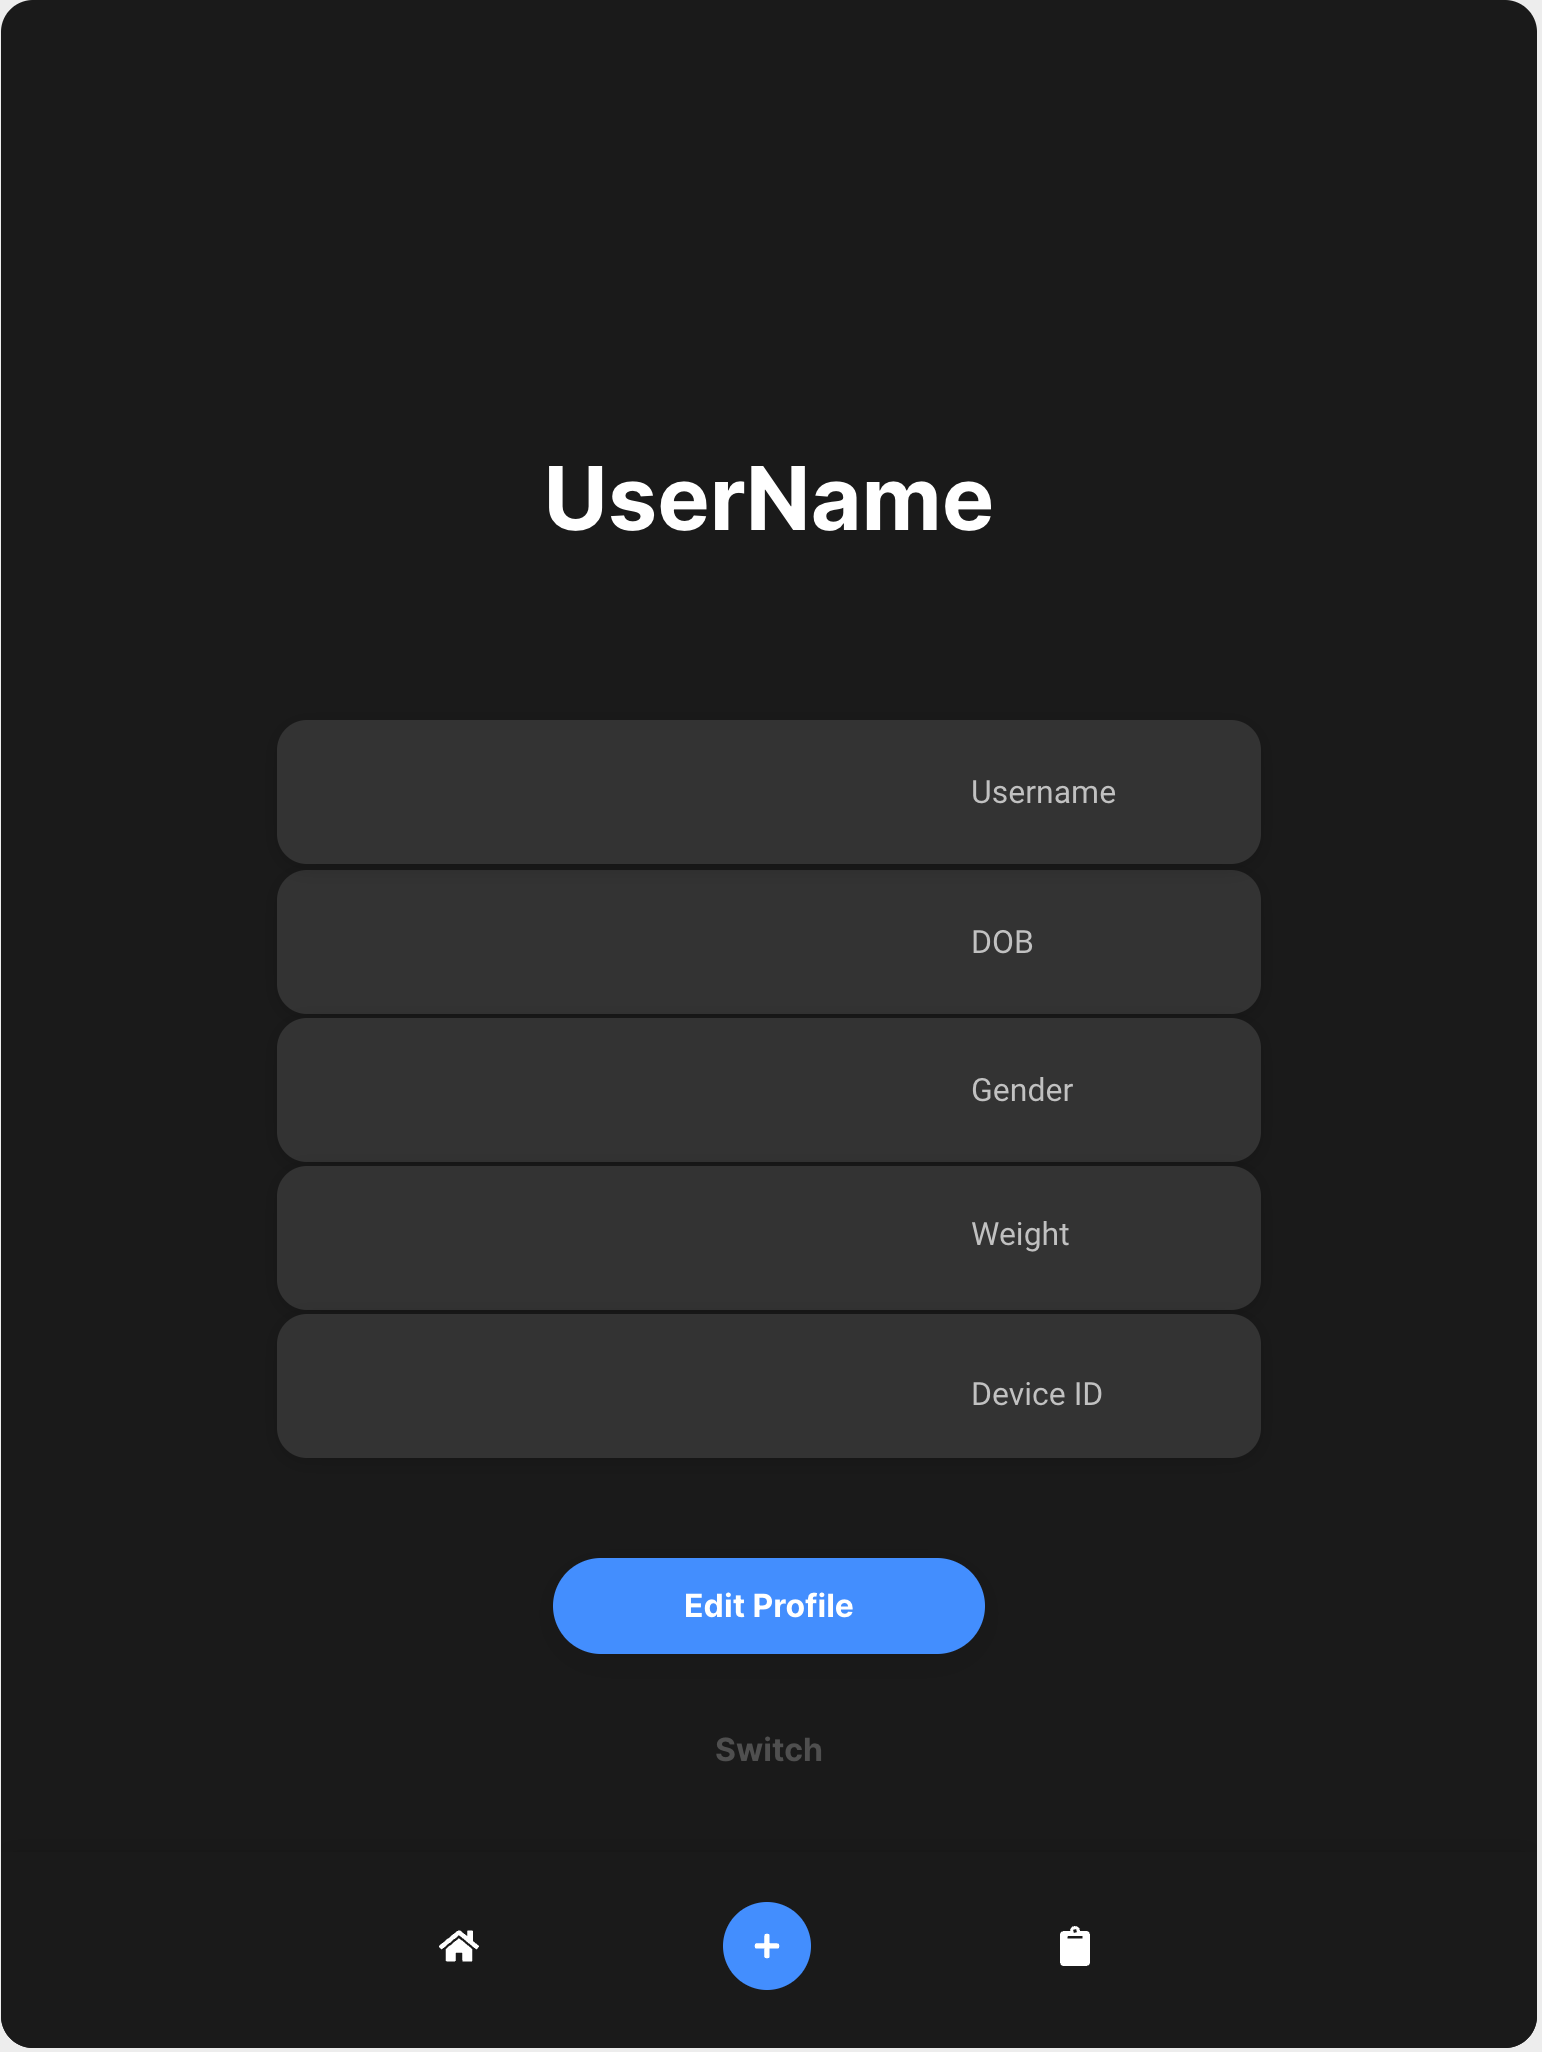
\includegraphics[width=0.75\textwidth]{images/user-fragment-mockup.png}
    \caption{UserFragment mock-up}
    \label{fig:userfragment_mockup}
\end{figure}

To fulfill the requirements, the \emph{UserFragment} must facilitate adding a new user and updating their data. The functionalities to add a new user and to update their data share the same sequence of operations in the \emph{view} level with the only difference is the button.
As a result, the following sequence of operations is created to support the functionality to add a new user and to update their data.

\begin{enumerate}
    \item A button to add new user or update user is pressed.
    \item User data is retrieved from the input and validated.
    \item User data sent to \emph{UserViewModel} to be persisted in the database.
    \item Saved user is returned
    \item The UI is updated according to the saved user.
\end{enumerate}

\begin{figure}[H]
    \centering
    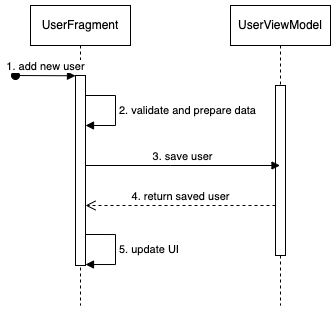
\includegraphics[width=0.5\textwidth]{diagrams/create-user-seq.drawio.png}
    \caption{UserFragment add new user sequence diagram}
    \label{fig:userfragment_add new user}
\end{figure}

To meet the requirement of deleting user data, the UserFragment is designed to handle this functionality. 
To support this functionality, the following sequence of operation is implemented:
